\documentclass[10pt,a4paper]{article}                                         
\usepackage{CJKutf8}                                                          
\usepackage{inputenc}                                                         
\usepackage[T1]{fontenc}                                                      
\usepackage{amsmath,esint}                                                    
\usepackage{amsfonts}                                                         
\usepackage{amssymb}                                                          
\usepackage{xcolor}                                                           
\usepackage{mathrsfs}                                                         
\usepackage{makeidx}                                                          
\usepackage{graphicx}                                                         
\usepackage{float}                                                            
\usepackage{textcomp}                                                         
\usepackage{gensymb}                                                          
\usepackage{ifpdf}                                                            
\usepackage{tikz}                                                             
\usepackage[siunitx]{circuitikz}                                              
\usetikzlibrary{shapes,arrows,positioning}                                    
%\usepackage{tgothic}                                                         
\ifpdf                                                                        
\usepackage[breaklinks,hidelinks]{hyperref}                                   
\else                                                                         
\usepackage{url}                                                              
\fi                                                                           
%\newcommand*\VF[1]{\mathbf{#1}}                                              
%\newcommand*\dif{\mathop{}\!\mathrm{d}}                                      
\author{CBCO}                                                           
\title{Block Diagram in LaTeX Tikz}                                                             
\begin{document}                                                              
\maketitle

\noindent \newcommand\CWht[1][2.5]{\tikz[baseline=-#1]{\draw[thick](0,0)     circle[radius=1.5mm];}}
 \par \ \par\noindent \newcommand\CBlk[1][2.5]{\tikz[baseline=-#1]{\draw[thick,    fill=black!](0,0) circle[radius=1.5mm];}}
 \par \ \par\noindent \begin{CJK*}{UTF8}{gbsn}
 \par \ \par\noindent \section{Block Diagrams }
 \par \ \par\noindent The typical control system diagram in Figure 1 was drawn using \href{ https://tex.stackexchange.com/questions/175969/block-diagrams-using-tikz}{Tikz}. The Figure 1 (a) was basic control system. The Figure 1 (b) was the simplification of Figure 1 (a). 

 \par \ \par\noindent \begin{figure}[H] \centering 

 \par \ \par\noindent \tikzstyle{block}=[draw, fill=white, rectangle,                             
minimum height=3em,minimum width=6em]                                        
\tikzstyle{sum} = [draw, fill=white, circle, node distance=1cm]             
\tikzstyle{input} = [coordinate]                                            
\tikzstyle{output} = [coordinate]                                           
\tikzstyle{pinstyle} = [pin edge={to-,thin,black}]                          
\begin{tikzpicture}[auto, node distance=2cm,>=latex']                       
%(a)                                                                         
\node [input, name=input] {};                                               
\node [sum, right of=input] (sum) {};                                       
\node [block, right of=sum] (controller) {Controller};                      
\node [block, right of=controller, pin={[pinstyle]above:D},                 
            node distance=3cm] (system) {System};                            
\draw [->] (controller) -- node[name=u] {$u$} (system);                     
\node [output, right of=system] (output) {};                                
\node [block, below of=u] (measurements) {Measurements};                    
\draw [draw,->] (input) -- node {$r$} (sum);                                
\draw [->] (sum) -- node {$e$} (controller);                                
\draw [->] (system) -- node [name=y] {$y$}(output);                         
\draw [->] (y) |- (measurements);                                           
\draw [->] (measurements) node [below=1cm ]{$(a)$} -| node[pos=0.99] {$-$}  
        node [near end] {$y_m$} (sum) ;                                      
%(b)                                                                         
\node [input, below of =input, node distance = 5cm](input1) {};             
\node [sum, right of=input1] (sum1) {};                                     
\node [block, right of=sum1, node distance = 3.5cm]                         
    (feedforward) {Feedforward=Ff};                                          
\node [output, right of=feedforward, node distance = 3cm] (output1) {};     
\node [block, below of=feedforward] (feedback) {Feedback=Fb};               
\draw [draw,->] (input1) -- node {$r$} (sum1);                              
\draw [->] (sum1) -- node {$e$} (feedforward)                               
    -- node [name=y1] {$y$}(output1);                                        
\draw [->] (output1) |- (feedback);                                         
\draw [->] (feedback) node [below=1cm ]{$(b)$} -| node[pos=0.99] {$-$}      
        node [near end] {$y_m$} (sum1) ;                                     
\node [input, below of =input, node distance = 5cm](input1) {};             
\node [sum, right of=input1] (sum1) {};                                     
\node [block, right of=sum1, node distance = 3.5cm]                         
    (feedforward) {Feedforward=Ff};                                          
\node [output, right of=feedforward, node distance = 3cm] (output1) {};     
\node [block, below of=feedforward] (feedback) {Feedback=Fb};               
\draw [draw,->] (input1) -- node {$r$} (sum1);                              
\draw [->] (sum1) -- node {$e$} (feedforward)                               
    -- node [name=y1] {$y$}(output1);                                        
\draw [->] (output1) |- (feedback);                                         
\draw [->] (feedback) node [below=1cm ]{$(b)$} -| node[pos=0.99] {$-$}      
        node [near end] {$y_m$} (sum1) ;                                     
\end{tikzpicture} 
 \par \ \par\noindent \caption{Block diagram}
    \end{figure}

 \par \ \par\noindent \par \ \par
 \par \ \par\noindent Consider Figure 1 (b). The following equations were noted. Note that the    negative sign in sum means negative feedback. 
 \par \ \par\begin{equation}
 \begin{minipage}{250pt}
                \begin{flushleft} $\displaystyle e = r - y_{m}$  \end{flushleft}
 \end{minipage}
 \end{equation}
\begin{equation}
 \begin{minipage}{250pt}
                \begin{flushleft} $\displaystyle y_{m} = F_{b} y$  \end{flushleft}
 \end{minipage}
 \end{equation}
\begin{equation}
 \begin{minipage}{250pt}
                \begin{flushleft} $\displaystyle y = F_{f} e$  \end{flushleft}
 \end{minipage}
 \end{equation}
\noindent Eliminating e, and ym 
 \par \ \par\begin{equation}
 \begin{minipage}{250pt}
                \begin{flushleft} $\displaystyle y = F_{f} \left(- F_{b} y + r\right)$  \end{flushleft}
 \end{minipage}
 \end{equation}
\begin{equation}
 \begin{minipage}{250pt}
                \begin{flushleft} $\displaystyle y \left(F_{b} F_{f} + 1\right) = F_{f} r$  \end{flushleft}
 \end{minipage}
 \end{equation}
\begin{equation}
 \begin{minipage}{250pt}
                \begin{flushleft} $\displaystyle y = \frac{F_{f} r}{F_{b} F_{f} + 1} = \frac{r}{F_{b} + \frac{1}{F_{f}}}$  \end{flushleft}
 \end{minipage}
 \end{equation}
\begin{equation}
 \begin{minipage}{250pt}
                \begin{flushleft} $\displaystyle y \approx \frac{1}{F_b}r \quad for 1 << F_f$  \end{flushleft}
 \end{minipage}
 \end{equation}
\noindent The open loop gain was feedforward. The close loop gain was reciprocal of    feedback. If Fb = 1, then y=r. It was called unity feedback. Current mirrors    made used of unity feedback. 
 \par \ \par\noindent \section{Block Diagrams of Schematic Passive Circuit Components}
 \par \ \par\noindent \subsection{Resistor}
 \par \ \par\noindent \begin{figure}[H] \centering 

 \par \ \par\noindent \begin{circuitikz}[american]   
\draw (0,0) to[isource, l=$I_{in}$] (0,3) -- (2,3) 
to[R=$R$, v=$V_{out}$, i=$i_{in}$] (2,0) -- (0,0) 
node[left, below=2cm]{$\hspace{2cm}(a)$}; 
\draw (0,0) -- (0,-1 )node[ground]{};
\end{circuitikz}
 \par \ \par\noindent \begin{circuitikz}[american]   
\draw (0,0) to[vsource, V=$V_{in}$] (0,3) -- 
(2,3) 
to[R=$R$, v=$V_{in}$, i=$i_{out}$] (2,0) -- (0,0)
node[left, below=2cm]{$\hspace{2cm}(c)$}; 
\    ; 
\draw (0,0) -- (0,-1 )node[ground]{};
\end{circuitikz}
 \par \ \par\noindent \par \ \par
 \par \ \par\noindent \hspace{.5cm}
\tikzstyle{block} = [draw, fill=white, rectangle,                             
    minimum height=3em, minimum width=6em]                                     
\tikzstyle{input} = [coordinate]                                              
\tikzstyle{output} = [coordinate]                                             
\begin{tikzpicture}[auto, node distance=2cm,>=latex']                         
\node [input, above = 2cm,  name=in] {};                                      
\node [block, right of=in] (iv) {$v_{out}=R*i_{in}$};                         
\node [output, right of=iv] (out) {$v_{out}$};                                
\draw [->] (in)  -- node {$i_{in}$} (iv);                                     
\draw [->] (iv) node[below=.75cm]{$(b)$}-- node [name=v] {$v_{out}$}(out);    
\end{tikzpicture}\hspace{.5cm}
 \par \ \par\noindent \tikzstyle{block} = [draw, fill=white, rectangle,                             
    minimum height=3em, minimum width=6em]                                     
\tikzstyle{input} = [coordinate]                                              
\tikzstyle{output} = [coordinate]                                             
\begin{tikzpicture}[auto, node distance=2cm,>=latex']                         
\node [input, above = 2cm,  name=in] {};                                      
\node [block, right of=in] (iv) {$i_{out}=R^{-1}*v_{in}$};                    
\node [output, right of=iv] (out) {$i_{out}$};                                
\draw [->] (in)  -- node {$v_{in}$} (iv);                                     
\draw [->] (iv) node[below=.75cm]{$(d)$}-- node [name=i] {$i_{out}$}(out);    
\end{tikzpicture}
 \par \ \par\noindent \caption{Resistor Circuits schematic to Resistor blocks diagram}          
    \end{figure}

 \par \ \par\noindent \par \ \par
 \par \ \par\noindent The resistor schematic circuit diagram was shown in Figure 2 (a). It had a     current source as input. Its block diagram was shown in Figure 2 (b). The     resistor schematic circuit diagram with voltage source as input was shown     in Figure 2 (c). 
 \par \ \par\noindent The equations of Resistor in time domain were the following.
 \par \ \par\begin{equation}
 \begin{minipage}{250pt}
                \begin{flushleft} $\displaystyle v_{out}{\left(t \right)} = R i_{in}{\left(t \right)}$  \end{flushleft}
 \end{minipage}
 \end{equation}
\begin{equation}
 \begin{minipage}{250pt}
                \begin{flushleft} $\displaystyle i_{in}{\left(t \right)} = \frac{v_{out}{\left(t \right)}}{R}$  \end{flushleft}
 \end{minipage}
 \end{equation}
\noindent \subsection{Capacitor}
 \par \ \par\noindent \begin{figure}[H] \centering 

 \par \ \par\noindent \begin{circuitikz}[american]                                              
\draw (0,0) to[isource, l=$I_{in}$] (0,3) --(2,3) 
to[C=$C$, v=$V_{out}$, i=$i_{in}$] (2,0) -- (0,0) 
node[left, below=2cm]{$\hspace{2cm}(a)$}; 
\draw (0,0) -- (0,-1 )node[ground]{};
\end{circuitikz}
 \par \ \par\noindent \begin{circuitikz}[american]   
\draw (0,0) to[vsource, V=$V_{in}$] (0,3) -- 
(2,3) 
to[C=$C$, v=$V_{in}$, i=$i_{out}$] (2,0) -- (0,0)
node[left, below=2cm]{$\hspace{2cm}(a)$}; 
\draw (0,0) -- (0,-1 )node[ground]{};
\end{circuitikz}
 \par \ \par\noindent \par \ \par
 \par \ \par\noindent \hspace{.5cm}
\tikzstyle{block} = [draw, fill=white, rectangle,                           
    minimum height=3em, minimum width=6em]                                   
\tikzstyle{input} = [coordinate]                                            
\tikzstyle{output} = [coordinate]                                           
\begin{tikzpicture}[auto, node distance=2cm,>=latex']                       
\node [input, above = 2cm,  name=in] {};              
\node [block, right of=in] (iv) {$v_{out}=C^{-1}\int{i_{in}dt}$};                               
\node [output, right of=iv] (out) {$v_{out}$};                                 
\draw [->] (in)  -- node {$i_{in}$} (iv);                                      
\draw [->] (iv) node[below=.75cm]{$(b)$}-- node [name=v] {$\hspace{.5cm}v_{out}$}(out);                                  
\end{tikzpicture}\hspace{.5cm}
 \par \ \par\noindent \tikzstyle{block} = [draw, fill=white, rectangle,                             
    minimum height=3em, minimum width=6em]                                     
\tikzstyle{input} = [coordinate]                                              
\tikzstyle{output} = [coordinate]                                             
\begin{tikzpicture}[auto, node distance=2cm,>=latex']                         
\node [input, above = 2cm,  name=in] {};                                      
\node [block, right of=in] (iv) {$i_{out}=C\frac{dv_{in}}{dt}$};             
\node [output, right of=iv] (out) {$i_{out}$};                                
\draw [->] (in)  -- node {$v_{in}$} (iv);                                     
\draw [->] (iv) node[below=.75cm]{$(d)$}-- node [name=i] {$i_{out}$}(out);    
\end{tikzpicture}
 \par \ \par\noindent \caption{Capacitor Circuits schematic to Capacitor blocks diagram}
    \end{figure}

 \par \ \par\noindent \par \ \par
 \par \ \par\noindent The schematic circuit diagram of capacitor with current source as input     was shown in Figure 3 (a). Its block diagram was shown in Figure 3 (b).     Its schematic circuit diagram with voltage source as input was shown in     Figure 3 (c). Its block diagram was shown in Figure 3 (d). The capacitor     equations were expressed as follows.
 \par \ \par\begin{equation}
 \begin{minipage}{250pt}
                \begin{flushleft} $\displaystyle v_{out}{\left(t \right)} = \frac{\int i_{in}{\left(t \right)}\, dt}{C}$  \end{flushleft}
 \end{minipage}
 \end{equation}
\begin{equation}
 \begin{minipage}{250pt}
                \begin{flushleft} $\displaystyle i_{in}{\left(t \right)} = C \frac{d}{d t} v_{out}{\left(t \right)}$  \end{flushleft}
 \end{minipage}
 \end{equation}
\noindent \subsection{Inductor}
 \par \ \par\noindent \begin{figure}[H] \centering 

 \par \ \par\noindent \begin{circuitikz}[american]                                              
\draw (0,0) to[isource, l=$I_{in}$] (0,3) -- (2,3)                             
to[L=$L$, v=$V_{out}$, i=$i_{in}$] (2,0) -- (0,0)                              
node[left, below=2cm]{$\hspace{2cm}(a)$};                                      
\draw (0,0) -- (0,-1 )node[ground]{};                                          
\end{circuitikz}
 \par \ \par\noindent \begin{circuitikz}[american]                                              
\draw (0,0) to[vsource, V=$V_{in}$] (0,3) -- (2,3)                             
to[L=$L$, v=$V_{in}$, i=$i_{out}$] (2,0) -- (0,0)                              
node[left, below=2cm]{$\hspace{2cm}(a)$};                                      
\draw (0,0) -- (0,-1 )node[ground]{};                                          
\end{circuitikz}
 \par \ \par\noindent \par \ \par
 \par \ \par\noindent \hspace{.5cm}
\tikzstyle{block} = [draw, fill=white, rectangle,                             
    minimum height=3em, minimum width=6em]                                     
\tikzstyle{input} = [coordinate]                                              
\tikzstyle{output} = [coordinate]                                             
\begin{tikzpicture}[auto, node distance=2cm,>=latex']                         
\node [input, above = 2cm,  name=in] {};                                      
\node [block, right of=in] (iv) {$v_{out}=L\frac{i_{in}}{dt}$};              
\node [output, right of=iv] (out) {$v_{out}$};                                
\draw [->] (in)  -- node {$i_{in}$} (iv);                                     
\draw [->] (iv) node[below=.75cm]{$(b)$}-- node [name=v]     {$\hspace{.5cm}v_{out}$}(out);                                            
\end{tikzpicture}\hspace{.5cm}
 \par \ \par\noindent \tikzstyle{block} = [draw, fill=white, rectangle,                             
    minimum height=3em, minimum width=6em]                                     
\tikzstyle{input} = [coordinate]                                              
\tikzstyle{output} = [coordinate]                                             
\begin{tikzpicture}[auto, node distance=2cm,>=latex']                         
\node [input, above = 2cm,  name=in] {};                                      
\node [block, right of=in] (iv) {$i_{out}=L\int{dv_{in}}{dt}$};              
\node [output, right of=iv] (out) {$i_{out}$};                                
\draw [->] (in)  -- node {$v_{in}$} (iv);                                     
\draw [->] (iv) node[below=.75cm]{$(d)$}-- node [name=i] {$i_{out}$}(out);    
\end{tikzpicture}
 \par \ \par\noindent \caption{Inductor Circuits schematic to Inductor blocks diagram}
    \end{figure}

 \par \ \par\noindent \par \ \par
 \par \ \par\noindent The schematic circuit diagram of inductor with current source as input     was shown in Figure 3 (a). Its block diagram was shown in Figure 3 (b).     Its schematic circuit diagram with voltage source as input was shown in     Figure 3 (c). Its block diagram was shown in Figure 3 (d). The inductor     equations were expressed as follows.
 \par \ \par\begin{equation}
 \begin{minipage}{250pt}
                \begin{flushleft} $\displaystyle v_{out}{\left(t \right)} = L \frac{d}{d t} i_{in}{\left(t \right)}$  \end{flushleft}
 \end{minipage}
 \end{equation}
\begin{equation}
 \begin{minipage}{250pt}
                \begin{flushleft} $\displaystyle i_{in}{\left(t \right)} = \frac{\frac{d}{d t} v_{out}{\left(t \right)}}{L}$  \end{flushleft}
 \end{minipage}
 \end{equation}
\noindent \section{Emitter Follower}
 \par \ \par\noindent \begin{figure}[H] \centering 

 \par \ \par\noindent \begin{circuitikz}[american]                                              
\draw (0,0) to[vsource=$V_{ref}$](0,3);                                        
\draw (4,0) to[R=$R_e$](4,3);                                                  
\draw (0,0) --(0,-.5) node[ground]{};                                          
\draw (4,0) --(4,-.5) node[ground]{};                                          
\draw (4,4) node[npn](npn1){Q1};                                               
\draw (4,5) to[R=$R_c$](4,8);                                                  
\draw (7,9) to[vsource=$V_{cc}$](7,5);                                         
\draw (7,5) --(7, 5) node[ground]{};                                           
\draw (4,8) |- (7,9);                                                          
\draw [->] (npn1.C) -- (4,5) node[midway]{}--(5,5)node[]{$\hspace{.5cm} V_c$};
\draw (npn1.E) -- (4,3) -- (5,3) node[]{$\hspace{.5cm}V_e$};                   
\draw (npn1.B) -| (0,3)node[left]{$V_{ref}$};                                  
\draw (3.5,3.5) node[]{$V_{be}$};                                              
\end{circuitikz}
 \par \ \par\noindent \caption{Schematic Circuit diagram of emitter follower}                   
    \end{figure}

 \par \ \par\noindent \begin{figure}[H] \centering 

 \par \ \par\noindent 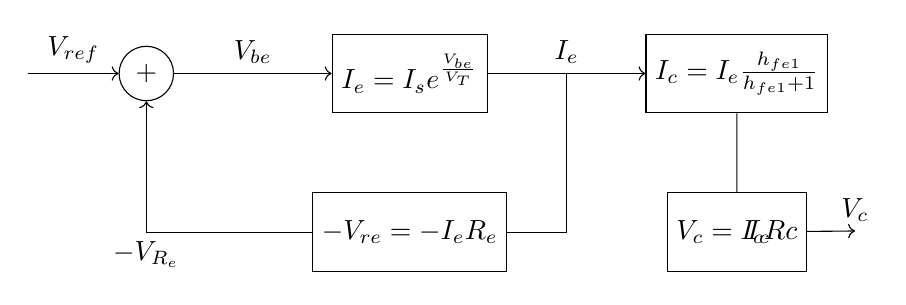
\begin{tikzpicture}                                                       
\node[draw, circle, minimum size=0.5cm] (sum1){+};                            
\node [draw,  minimum width=1cm, minimum height=1cm,                          
    right=2cm of sum1] (Q1e) {$I_e=I_se^{\frac{V_{be}}{V_T}}$};               
\node [draw,  minimum width=1cm, minimum height=1cm,                          
    below= of Q1e] (Re) {$-V_{re}=-I_eR_e$};                                   
\node [draw,  minimum width=1cm, minimum height=1cm,                          
    right= 2cm of Q1e] (Q1c) {$I_{c}=I_e\frac{h_{fe1}}{h_{fe1}+1}$};          
\node [draw, minimum width=1cm, minimum height =1cm,                          
    below = of Q1c](Rc){$V_c = I_c Rc$};                                       
\draw[->] ++(-1.5,0) --  (sum1.west) node[midway,above]{$V_{ref}$};           
\draw [->] (sum1) -- (Q1e)node[midway,above ]{$V_{be}$};                      
\draw [->] (Q1e)-- (Q1c)node[midway,above](m1){$I_e$};                        
\draw [->] (m1) |-(Re) -| (sum1.south) node[midway,below]{$-V_{R_e}$};        
\draw [->] (Q1c) -- (Rc)node[right]{$I_c$} -- (9cm,-2cm)node[above]{$V_c$};   
\end{tikzpicture}
 \par \ \par\noindent \caption{Control System Block Diagram of Emitter Follower Circuit of     Figure 8} \end{figure}

 \par \ \par\noindent \section{Block Diagram of current Mirrors}
 \par \ \par\noindent \subsection{Widlar Current Mirror}
 \par \ \par\noindent \begin{figure}[H] \centering 

 \par \ \par\noindent \begin{circuitikz}[american]                                              
\draw (2,0) node[npn,xscale=-1](npn1){Q1};                                     
\draw (npn1.E) --(2,-.5) node[ground]{};                                       
\draw (npn1.C) -| (npn1.B);                                                    
\draw (2,4) to[isource, ](2,2)--node[left]{$I_{in}$}(npn1.C);                  
\draw (2,4) -|  (3,3.5)node[ground]{};                                         
\draw (4,0) node[npn](npn2){Q2};                                               
\draw (npn1.B) --node[below]{$V_{be}$} (npn2.B);                               
\draw (npn2.E) --(4,-.5) node[ground]{};                                       
\draw (npn2.C) to[R=$R1$,](4,3) -|(6,2) to[vsource](6,0)--                     
      (6,-.5) node[ground]{};                                                  
\end{circuitikz}
 \par \ \par\noindent \caption{Widlar current mirror schematic diagram}                         
    \end{figure}

 \par \ \par\noindent \subsection{Wilson Current Mirror}
 \par \ \par\noindent \begin{figure}[H] \centering 

 \par \ \par\noindent \begin{circuitikz}[american]                                              
\draw (2,0) node[npn,xscale=-1](npn1){Q1};                                     
\draw (npn1.E) --(2,-.5) node[ground]{};                                       
\draw (2,6) to[isource, ](2,4)--node[left]{$I_{in}$}(npn1.C);                  
\draw (2,6) -|  (3,5.5)node[ground]{};                                         
\draw (4,0) node[npn](npn2){Q2};                                               
\draw (npn1.B) --node[below]{$V_{be}$} (npn2.B);                               
\draw (npn2.E) --(4,-.5) node[ground]{};                                       
\draw (4,2) node[npn](npn3){Q3};                                               
\draw (npn2.C) -| (npn2.B);                                                    
\draw (npn3.C) to[R=$R1$,](4,6) -|(6,2) to[vsource](6,0)--                     
      (6,-.5) node[ground]{};                                                  
\draw (npn3.E)-- (npn2.C);                                                     
\draw (2,2) -- (npn3.B);                                                       
\end{circuitikz}
 \par \ \par\noindent \caption{Wilson current mirror schematic diagram}
    \end{figure}

 \par \ \par\noindent \section{Exercises}
 \par \ \par\noindent 1. Write the Equations of Widlar current mirror. (5)
 \par \ \par\noindent 2. Draw the Widlar block diagram. (5) 
 \par \ \par\noindent 3. Write the equations of Wilson current mirror. (5)
 \par \ \par\noindent 4. Draw the block diagram of Wilson current mirror. (5)
 \par \ \par\noindent 5.There is a portion of Wilson current mirror that is Widlar current mirror. Draw the block diagram of Wilson current mirror incorporating a block that is the Widlar currrent mirror. (5)
 \par \ \par\noindent \nocite{2}
 \par \ \par\noindent \nocite{201}
 \par \ \par\noindent \nocite{202}
 \par \ \par\noindent \nocite{301}
 \par \ \par\noindent \nocite{310}
 \par \ \par\noindent \bibliographystyle{plain} 
 \bibliography{ccoLib/ccobib}
 \par \ \par\noindent \end{CJK*}
 \par \ \par\end{document}